\documentclass[12pt]{article}
\usepackage[english]{babel}
\usepackage[utf8x]{inputenc}
\usepackage{amsmath}
\usepackage{graphicx}
\usepackage[a4paper]{geometry}
\usepackage{float}

\begin{document}
\begin{titlepage}

% definition of custom command for horizontal lines
\newcommand{\HRule}{\rule{\linewidth}{0.5mm}}

\center
% HEADING
\textsc{\LARGE University of Dublin,\\Trinity College}\\[1.0cm]

\includegraphics[width=0.2\textwidth]{logo.png}

\HRule \\[0.4cm]
\textsc{\Large JS Engineering: 3C2 Digital Circuits}\\[0.25cm]
\textsc{\large D2: The MOS/CMOS Inverter}\\[0.1cm]
\HRule \\[0.4cm]
 
% AUTHORS
\begin{minipage}{0.5\textwidth}
\begin{flushleft} \large
\emph{Author:}
\\Edmond \textsc{O'Flynn} 12304742
\end{flushleft}
\end{minipage}
~
\begin{minipage}{0.4\textwidth}
\begin{flushleft} 
\large
\emph{Demonstrator:} \\
Cormac \textsc{Molloy} 
\end{flushleft}
\end{minipage}\\[3cm]

% DATE
{\large \today}\\[2cm] 

% LOGO
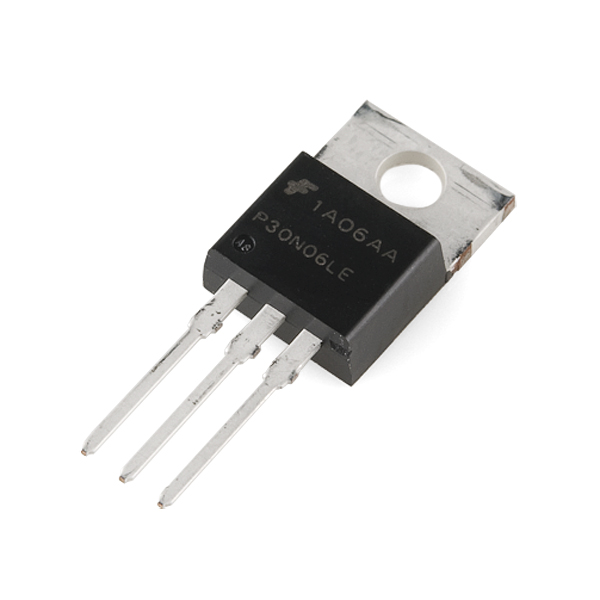
\includegraphics[width=0.2\textwidth]{mosfet.jpg}
\clearpage
\end{titlepage}

\newgeometry{top=2cm,left=2cm,bottom=2cm,right=2cm}

\tableofcontents
\thispagestyle{empty}
\cleardoublepage
\setcounter{page}{1}

\section{Abstract}
Lab D2 introduces the concept of MOS transistor simulation in the MultiSim 13.0 environment, and theory associated with the static and dynamic characteristics which show the effect of performance in various environments in the modern world of technology.
\section{Introduction}
The aim for this lab is to show and understand the differences between \emph{n-channel} and \emph{p-channel} MOS transistors, to test various properties of MOS, and also to demonstrate the performance of CMOS inverters. These states are modelled and examined during this laboratory through adjusting and viewing the properties associated with these states within circuit design.
\section{Theory}
\subsection{What is a MOSFET?}
MOSFETs are used in modern day technology to control electronics, similarly to a BJT. However a BJT controls by current, while a MOSFET is a voltage-controlled device that acts like a variable resistor, where voltage applied changes how the device conducts within the circuit. MOSFETs have a very high impedance, therefore it's extremely easy to drive on low current.
\subsection{How does a MOSFET work?}
A MOSFET is a voltage controlled field effect transistor that has its gate electrode highly insulated from the semiconductor in the transistor by a very thin layer of insulating material. The insulated metal gate acts similarly to how a capacitor's plate which causes an extremely high input resistance due to isolation. However, when a voltage is applied to the gate, the width of the \emph{drain-source} channel changes, and the device conducts freely. 

\begin{align*}
\centering

\includegraphics[width=0.25\textwidth]{mos.png}
\end{align*}
The main difference between a BJT and MOSFET is that a BJT is controlled by current, while a MOSFET is controlled by voltage. This implies that for a MOSFET, the output current is not a multiplier of the input due to MOSFETs pertaining to control by voltage.

\begin{align*}
\centering
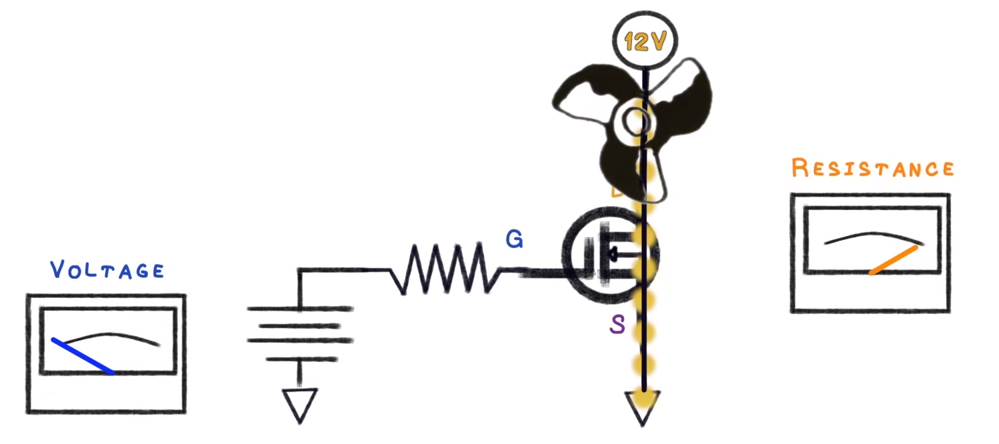
\includegraphics[width=0.5\textwidth]{mos-1.png}
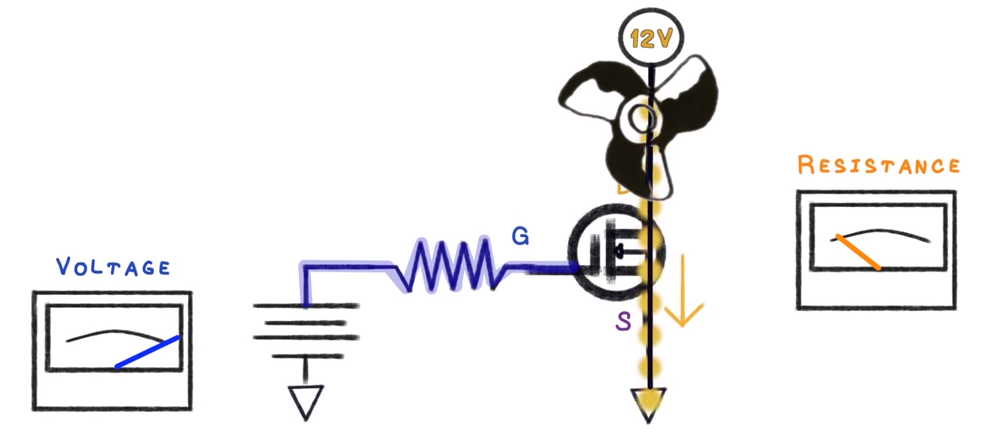
\includegraphics[width=0.5\textwidth]{mos-2.png}
\end{align*}
When current is applied between the gate and the source, current is allowed to flow from the drain to source. They are variable resistors controlled by voltage. Depending onthe voltage applied between the gate and source, the resistance between the gate and source will vary. With a low voltage between the gate and source, the resistance will be extremely high between the drain and source. As the voltage increases and a threshold is overcome, the resistance between the drain and source drops.

\subsection{How does a CMOS inverter work?}
CMOS stands for \emph{Complimentary Metal-Oxide Semiconductor}, which are some of the most widely used and adaptable MOSFET inverters used in a chip's design. They are noted to operate with very little power loss and at a very high speed, as well as having a good logic buffer with noise margins in its low and high states being large, and suitable for many applications.

\begin{align*}
\centering
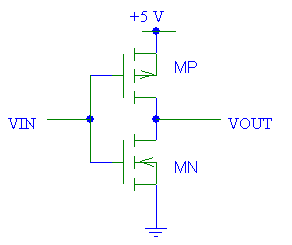
\includegraphics[width=0.5\textwidth]{cmos.png}
\end{align*}
A CMOS inverter contains both a P-MOS and N-MOS transistor connected at the drain and gate terminals of the semiconductor. A supply voltage V$_{DD}$ is connected at the P-MOS source terminal, and ground to the N-MOS's source pin. V$_{O}$ is connected to the transistors' drain terminals, and V$_{I}$ to the gate. CMOS does not contain any resistors, therefore it is far more power efficient than a MOSFET inverter in its regular state.

\subsection{Abbreviations}
\begin{itemize}
\item MOSFET
\begin{itemize}
\item MOSFET stands for \emph{Metal-Oxide Semiconductor Field Effect Transistor}, and is used to amplify signals or act as a switch in an electronic circuit. Their main advantage is the low current required (1mA) in order to activate, while delivering a much higher current load (10-50A).
\end{itemize}
\item N-channel
\begin{itemize}
\item An n-channel MOS transistor is classified as a semiconductor device where the electrons control the current flowing through it by utilising three terminal substrates: \emph{gate}, \emph{drain} and \emph{source}. These terminals allow for three different modes of operation that affect the output differently, whose modes are \emph{cut-off}, \emph{triode}, and \emph{saturation}. The n-channel generally has a lower resistance than a p-type MOS transistor. 
\end{itemize}
\item P-channel
\begin{itemize}
\item A p-type MOS transistor pertains to the same properties in terms of operation as a n-type MOS transistor, where the differences lie in its substrate composition, where the charge characteristics are holes instead of electrons.
\end{itemize}
\item Gate
\begin{itemize}
\item The gate is the terminal controlled by the voltage supplied to the MOS transistor.
\end{itemize}
\item Drain
\begin{itemize}
\item The drain is where the charge carriers can exit the channel.
\end{itemize}
\item Source
\begin{itemize}
\item The source is where the charge carriers can enter the channel.
\end{itemize}
\item $V_{GS}$
\begin{itemize}
\item This is the voltage that exists between the gate and source terminals.
\end{itemize}
\item $V_T$
\begin{itemize}
\item This is the threshold voltage of the transistor, other scripts such as O or I imply its threshold on the out- or input.
\end{itemize}
\item $V_{I}$
\begin{itemize}
\item This is the input voltage, other subscripts such as L or H determine the logic level implied.
\end{itemize}
\item $V_O$
\begin{itemize}
\item This is the output voltage, other subscripts such as L or H determine the logic level implied.
\end{itemize}
\item $V_{DD}$
\begin{itemize}
\item This is the positive power supply voltage that the circuit utilises to drive charge carriers.
\end{itemize}
\item $V_{IL MAX}$
\begin{itemize}
\item Max input voltage in order to recognise a logic LO.
\end{itemize}
\item $V_{IH MIN}$
\begin{itemize}
\item Minimum input voltage in order to recognise a logic HI
\end{itemize}
\item $V_{OL}$
\begin{itemize}
\item Output level to be recognised as a logical LO
\end{itemize}
\item $V_{OH}$
\begin{itemize}
\item Output level to be recognised as a logical HI
\end{itemize}
\item $R_{d}$
\begin{itemize}
\item Resistive load applied to the drain of the MOS transistor.
\end{itemize}
\item $t_{PHL}$
\begin{itemize}
\item The propagation delay that exists for an input changing from a logic high to a logic low.
\end{itemize}
\item $t_{PLH}$
\begin{itemize}
\item The propagation delay that exists for an input changing from a logic low to a logic high.
\end{itemize}
\item $t_{f}$
\begin{itemize}
\item The time taken for the voltage to cross the transistor junction in forward active mode.
\end{itemize}
\item $t_{r}$
\begin{itemize}
\item The time taken for the voltage to cross the transistor junction in reverse active mode.
\end{itemize}
\end{itemize}
\clearpage

\section{MOS Transistor Characteristics}
Using MultiSim 13.0, the following schematic should be drawn and connected up.
\subsection{Procedure}
\begin{figure}[H]
\centering
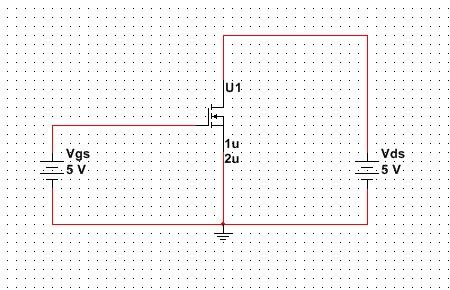
\includegraphics[width=0.5\textwidth]{2.jpg}
\caption{Drain Current v Gate-Source Voltage}
\end{figure}
\begin{itemize}
\item Create a new page and insert a N-MOS transistor with the following values onto the design schematic sheet. Ensure to save them to the user database for easy access.
\begin{itemize}
\item Length: $1\cdot10^{-4}$m
\item Width: $2\cdot10^{-4}$m
\item V$_{TO}$: 1V
\item $K_n$: $2\cdot10^{-5}$A/V${^2}$
\end{itemize}
\item Later on for a P-MOS transistor, the following values should be used instead, which should be also saved in the user database to save time.
\begin{itemize}
\item Length: $1\cdot10^{-4}$m
\item Width: $2\cdot10^{-4}$m
\item V$_{TO}$: -1V
\item $K_p$: $2\cdot10^{-5}$A/V${^2}$
\end{itemize}
\item Set up the schematic as shown in the diagram
\item Ensure the components are wired up correctly, including the ground.
\item Place a probe looking towards the drain of the MOS transistor
\item Perform a sweep using $V_{DS}$ as source 1, and $V_{GS}$ as source 2.
\item Also make sure that I(Probe1) has been added to the list of selected variables for analysis for generating a plot of I$_D$ v V$_{GS}$
\item On sweeping this, change the value of the MOS transistor width to 4$\mu$m and rerun the analysis.
\end{itemize}
\subsection{Results}
\begin{table}[H]
\centering
\begin{tabular}{lll}
       & N-Channel                                     & P-Channel                                      \\
Length & 0.0001m                                       & 0.0001m                                        \\
Width  & 0.0001m                                       & 0.0001m                                        \\
$V_{TO}$    & 1V                                            & -1V                                            \\
$K_p$, $K_n$  & $2\cdot10^{-5}$ A/V$^{2}$ & $1\cdot10^{-5}$ A/V$^{2}$
\end{tabular}
\caption{Reference Values}
\end{table}

\begin{figure}[H]
\centering
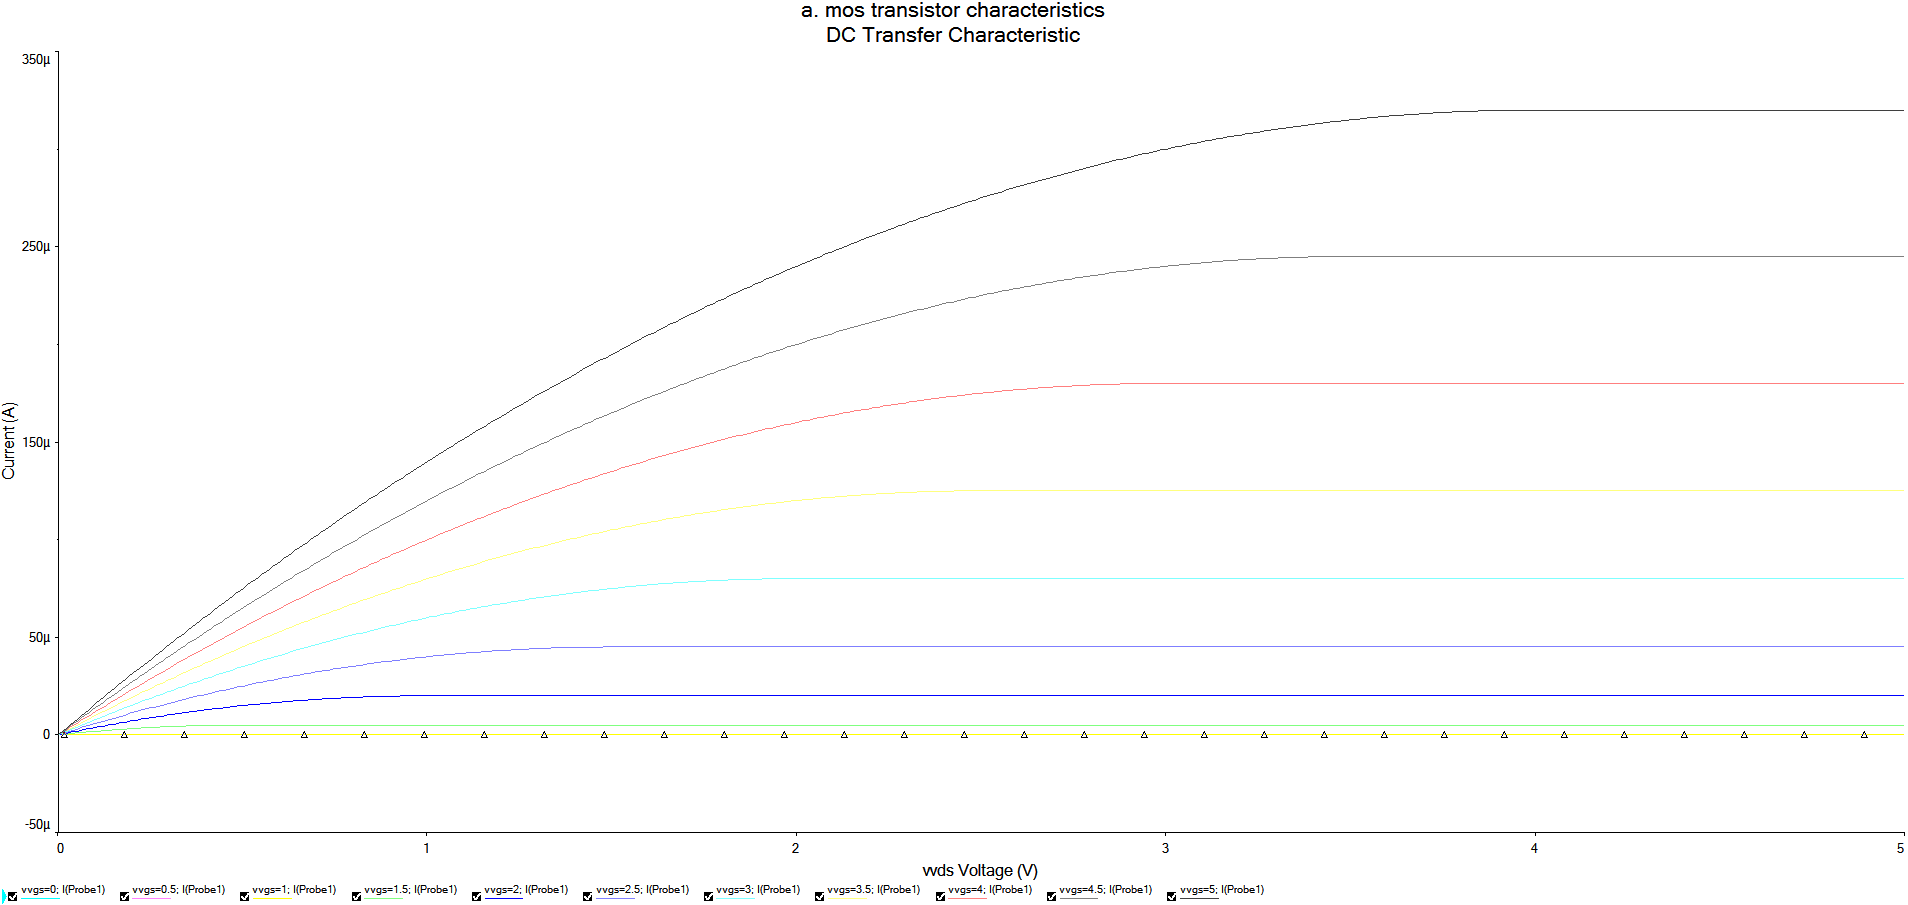
\includegraphics[width=0.9\textwidth]{a11.PNG}
\caption{MOS Transfer Characteristics at 2$\mu$m}
\end{figure}

\begin{figure}[H]
\centering
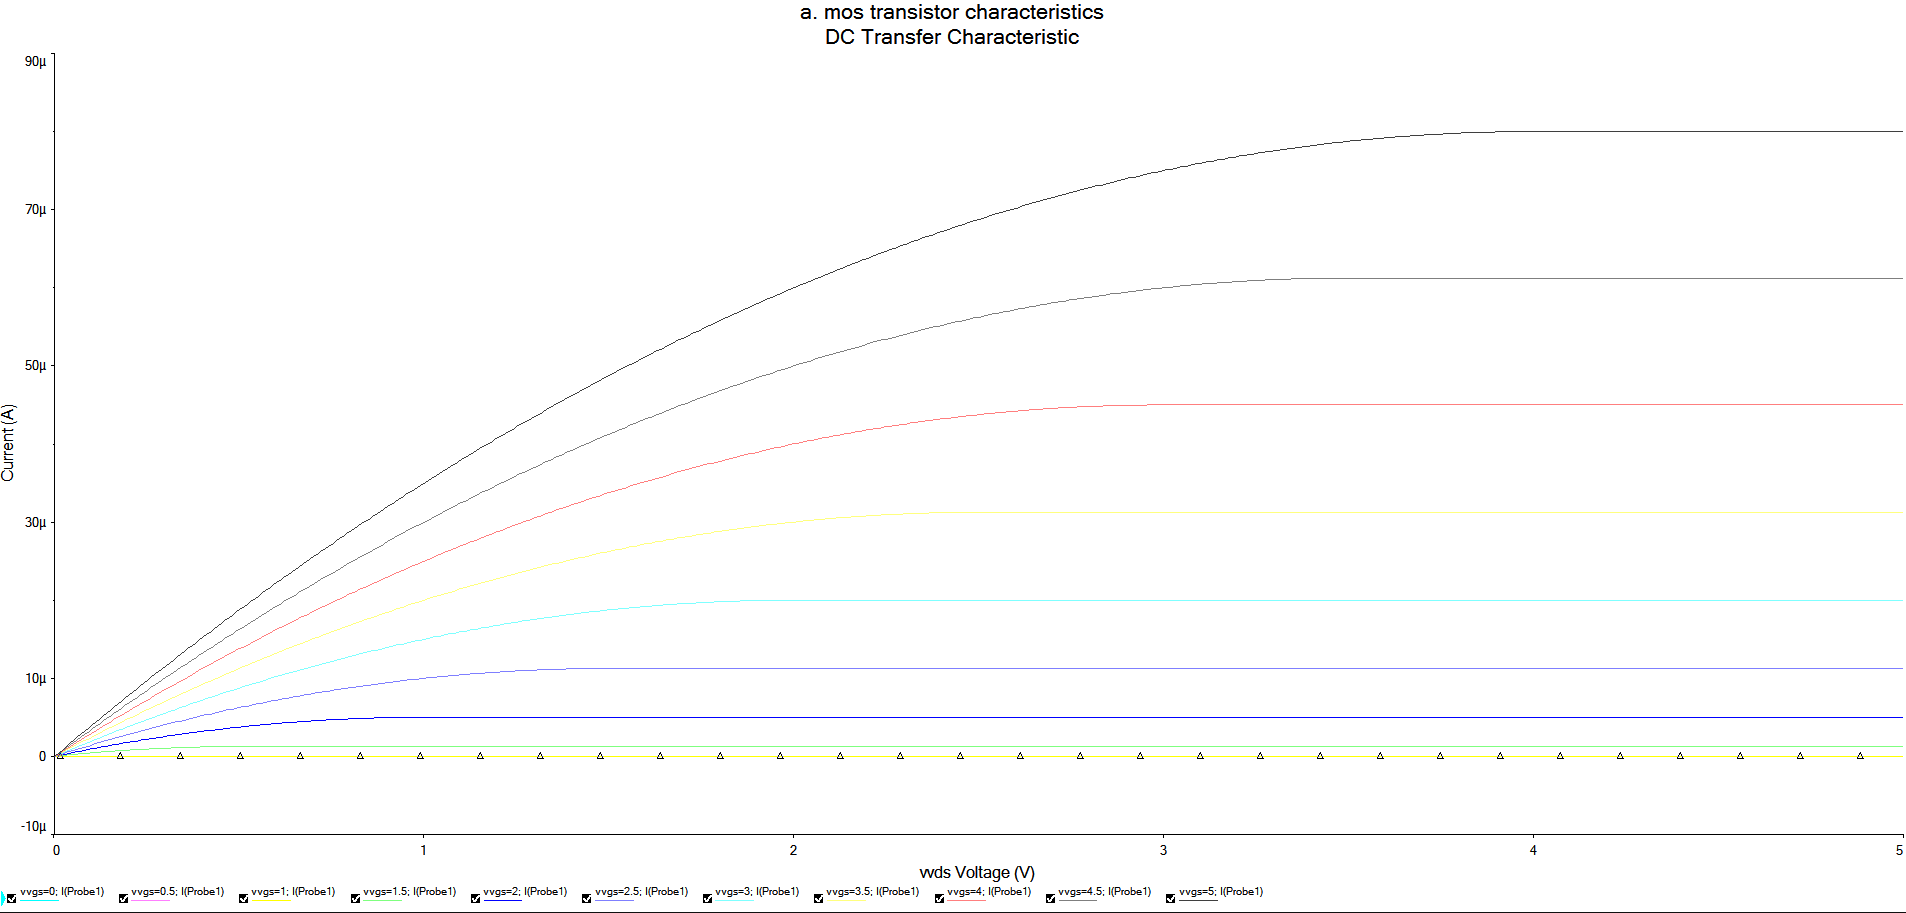
\includegraphics[width=0.9\textwidth]{a12.PNG}
\caption{MOS Transfer Characteristics at 4$\mu$m}
\end{figure}

\subsection{Discussion}
The sweep shows the effect of transitioning from the linear regime to the saturation mode of operation where channel debiasing begins to take effect. This transition changes from having more electrons in the channel as well as a stronger field pulling electrons from the source to a \emph{thinning down} from the source to drain as the current saturation of the drain-source approaches rapidly after a given point. The result of this is the levelling off effect of the voltage.

\section{Resistively Loaded MOS Transistor Inverter}
\subsection{Procedure}
\begin{figure}[H]
\centering
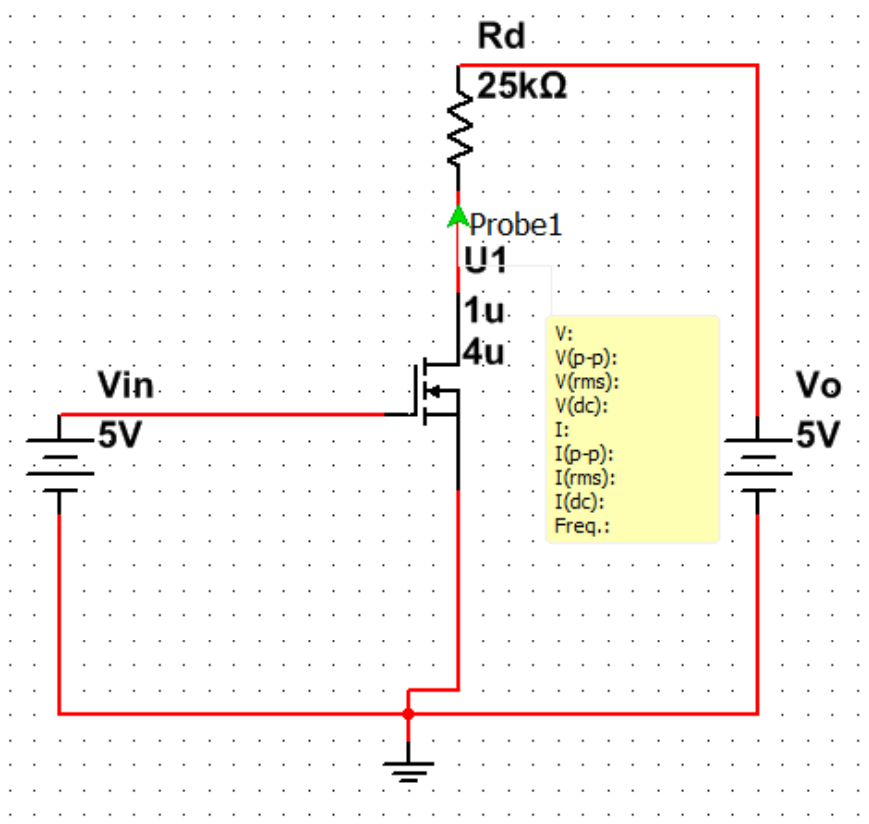
\includegraphics[width=0.4\textwidth]{b1.png}
\caption{Schematic}
\end{figure}
\begin{itemize}
\item Using the previously designed circuit, add the extra components to their respective positions by following the schematic provided.
\item When setting up a DC sweep, ensure that $V_{DS}$ is set to be source 1 instead of $V_{GS}$ where the probe is with respect to voltage, and not current.
\item When repeating the exercise, modify the resistor value $R_D$ to be 100k$\Omega$
\item Measure the logic values of $V_{IL MAX}$, $V_{IH MIN}$, $V_{OL}$, and $V_{OH}$ to be shown in the table below.
\end{itemize}
\subsection{Results}
Using the formula below, where $V_{GS}=V_{DD}$,
$$V_O=V_L=\left(V_{DD}-V_T+\frac{1}{K_nR_L}\right)\pm\sqrt{\left(V_{DD}-V_T+\frac{1}{K_nR_L}\right)^{2}-\frac{V_{DD}}{K_nR_L}}$$
We find that 100k$\Omega$ resistor has a $V_O$ of 7.44V or 0.305V, and the 25k$\Omega$ resistor has a $V_O$ of 8.87V or 1.127V.
\begin{table}[H]
\centering
\begin{tabular}{ll}
$V_{il max}$ & 1.51V \\
$V_{oh}$ & 5.05V \\
$V_{ih min}$ & 2.42V \\
$V_{ol}$ & 1.29V
\end{tabular}
\caption{25k$\Omega$ Resistor}
\end{table}

\begin{table}[H]
\centering
\begin{tabular}{ll}
$V_{il max}$ & 1.26V \\
$V_{oh}$ & 4.93V \\
$V_{ih min}$ & 1.17V \\
$V_{ol}$ & 645mV
\end{tabular}
\caption{100k$\Omega$ Resistor}
\end{table}

\begin{figure}[H]
\centering
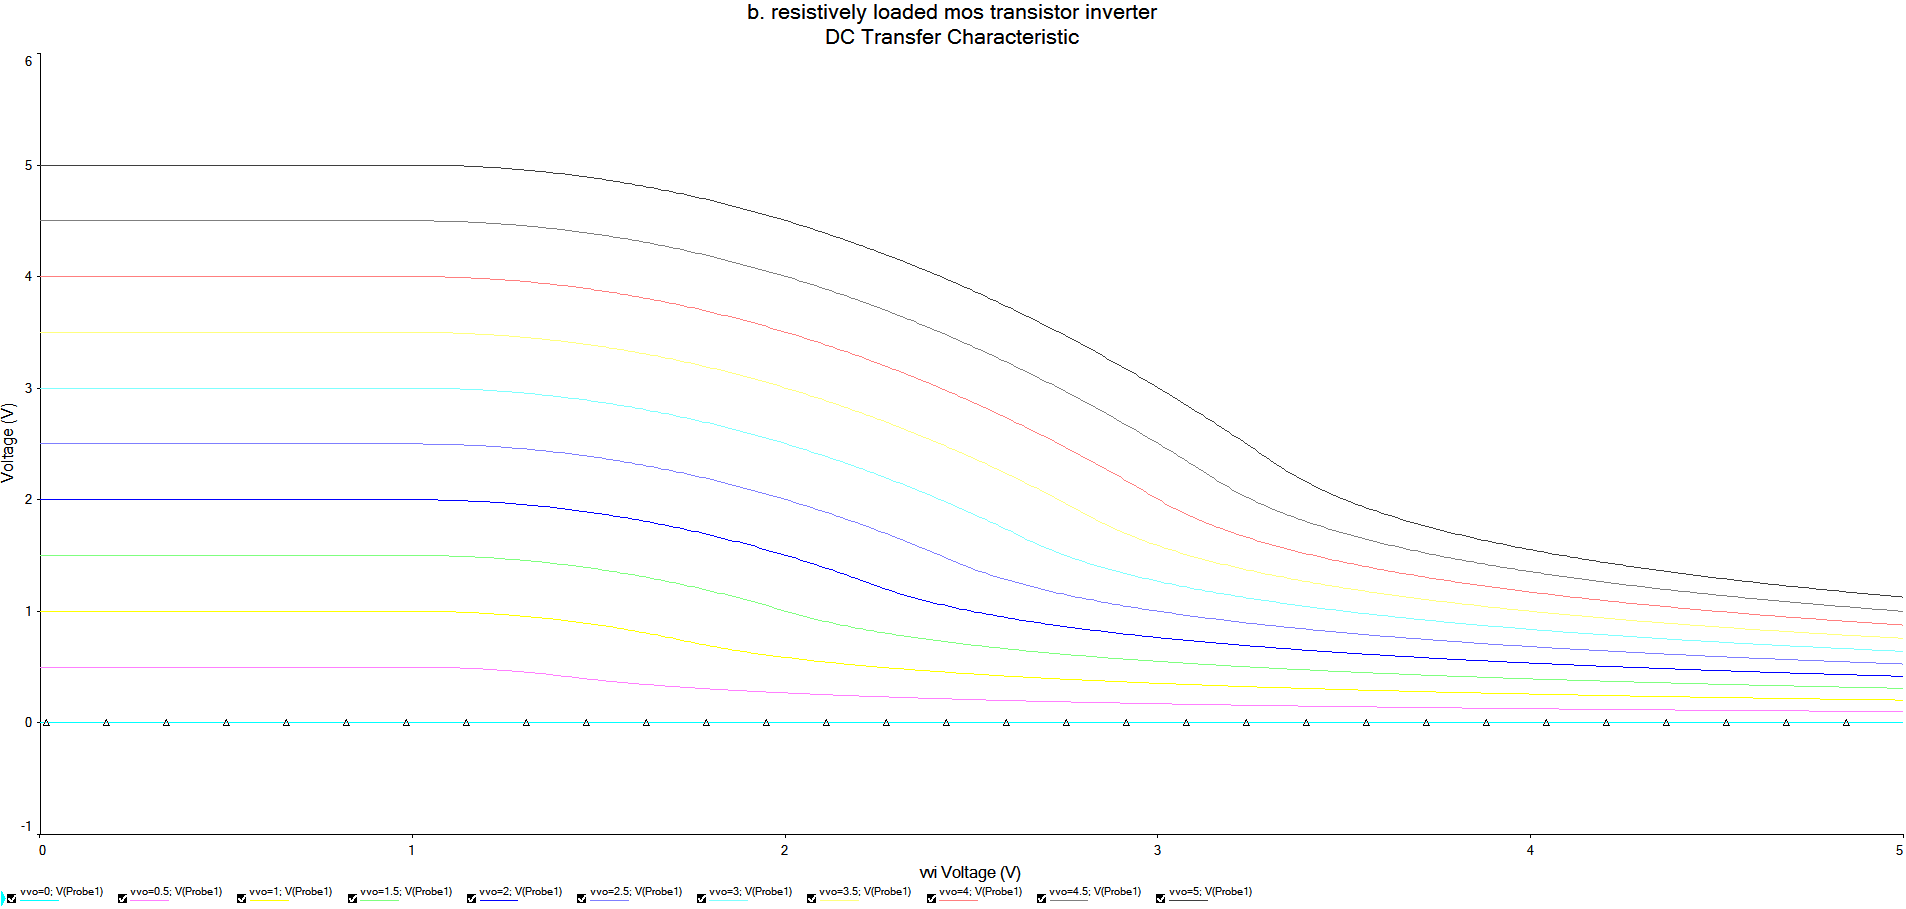
\includegraphics[width=1\textwidth]{b6.PNG}
\caption{Output of Sweep with 25k$\Omega$ resistor}
\end{figure}

\begin{figure}[H]
\centering
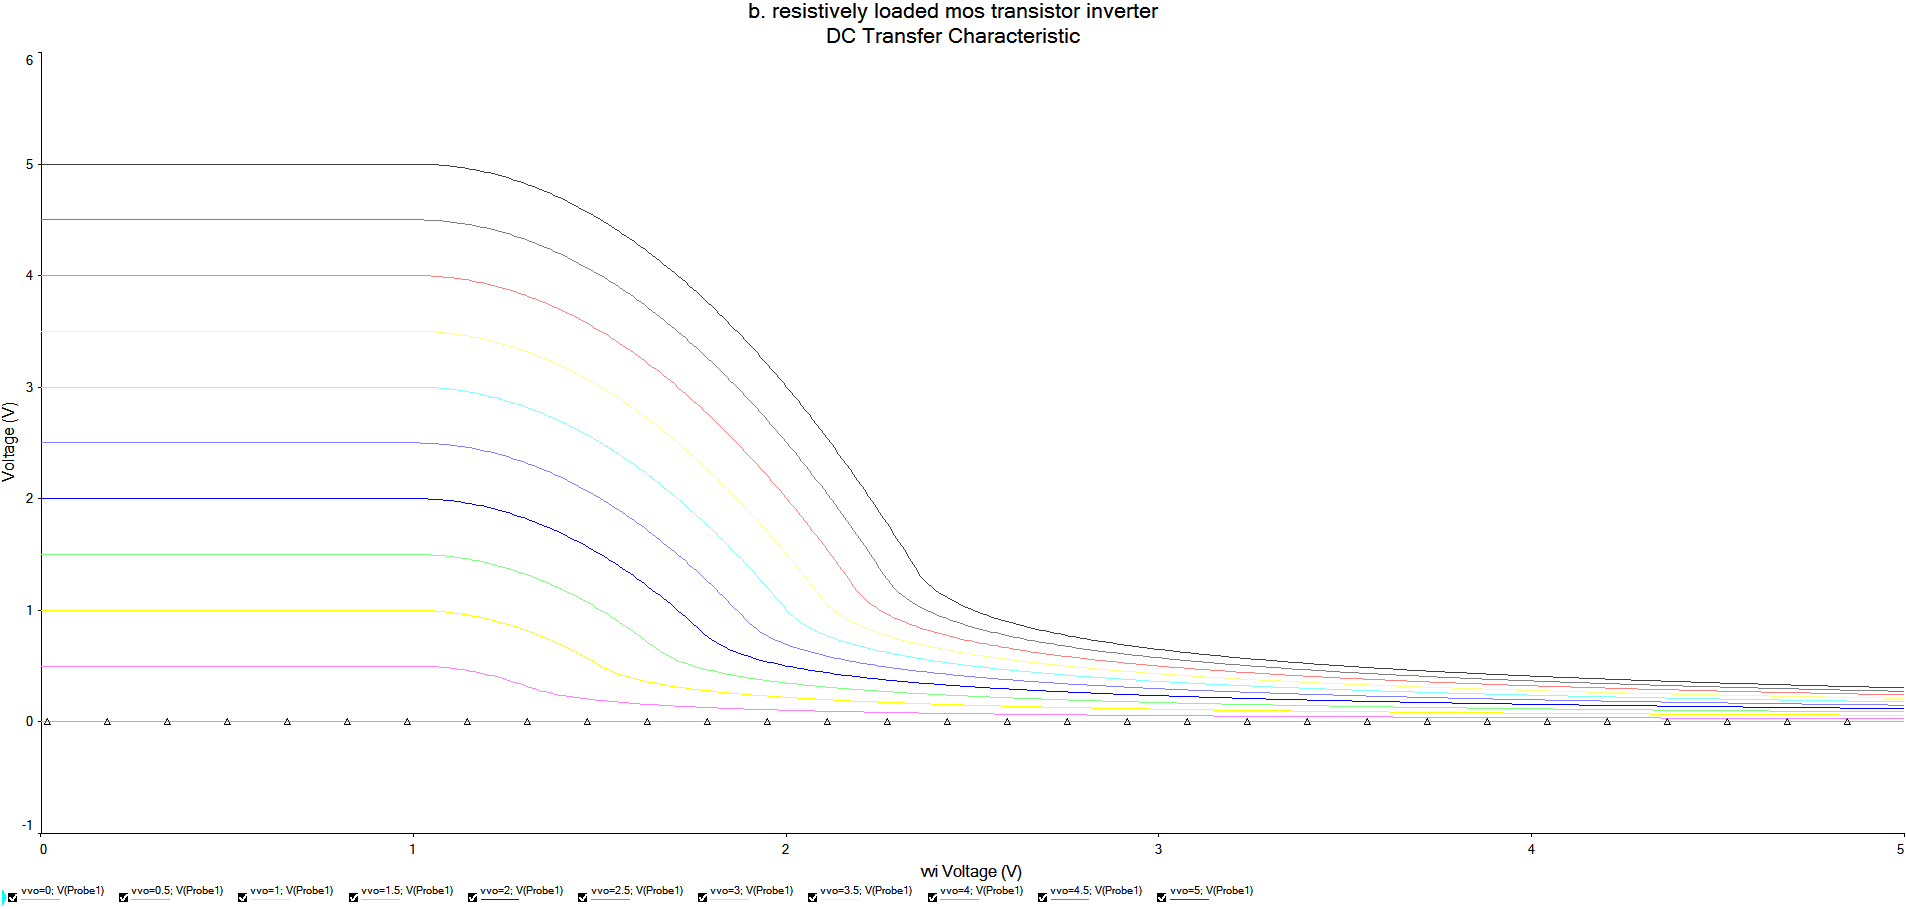
\includegraphics[width=1\textwidth]{b7.PNG}
\caption{Output of Sweep with 100k$\Omega$ resistor}
\end{figure}

\subsection{Discussion}
\begin{figure}[H]
\centering
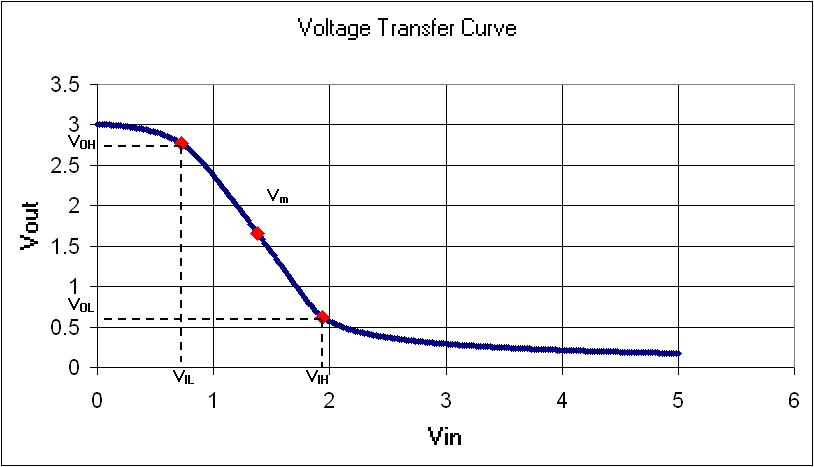
\includegraphics[width=0.5\textwidth]{4.jpg}
\caption{Voltage Transfer Characteristics}
\end{figure}

\begin{itemize}
\item The mode of operation within the transfer curve resides in three modes - cut-off, saturation and linear. Initially the current is negligible across the resistor, the same is also true for the voltage drop for the load within $V_{in}<V_{TO}$.
\item Next where $V_{TO}\leq V_{in}<V_{out}+V_{TO}$, the transistor enters saturation mode, where there is a noticeable increase in the input voltage, $V_{in}$, and a similar decrease in the output voltage, $V_{out}$.
\item Finally the transistor enters the linear stage of operation mode, where $V_{in} \geq V_{out} + V_{TO}$ which causes the output voltage to continue to decrease until its decrease tends to 0.
\end{itemize}

\subsubsection{Theoretical Calculations of $V_{OH}$ \& $V_{OL}$}
\begin{itemize}
\item Calculation of $V_{OH}$
\begin{itemize}
\item $V_{out}=V_{DD}-R_{L}I_{R}$
\item Where when the input voltage $V_{in}$ is low, $I_D=I_R=0$ which implies $V_{OH}=V_{DD}$
\end{itemize}
\item Calculation of $V_{OL}$
\begin{itemize}
\item Assuming that the input voltage is equivalent to $V_{OH}$, the linear region resides in $V_{in}-V_{TO} \geq V_{out}$
\item Given for the output node that $I_R=I_D$, $I_R=\frac{V_{DD}-V_{out}}{R_L}$
\item Where $\frac{V_{DD}-V_{OL}}{R_L}=\frac{k_n}{2} \cdot \left[ 2 \cdot (V_{DD} - V_{TO}) \cdot V_{OL} - V_{OL}^{2} \right]$
\item Such that $V_{OL}^{2} - 2 \cdot \left( V_{DD}-V_{TO}+\frac{1}{k_nR_L} \right) \cdot V_{OL} + \frac{2}{k_nR_L} \cdot V_{DD}$
\item Which results in $V_{OL}=V_{DD}-V_{TO}+\frac{1}{k_nR_L}-\sqrt{\left( V_{DD} - V_{TO} + \frac{1}{k_nR_L} \right)^{2} - \frac{2 V_{DD}}{k_nR_L}}$
\end{itemize}
\end{itemize}

\subsubsection{Theoretical Calculations of $V_{IL}$ \& $V_{IH}$}
\begin{itemize}
\item Calculation of $V_{IL}$
\begin{itemize}
\item By definition, $V_{IL}$ is the smaller of the two input voltages at which the slope, $\frac{dV_{out}}{dV_{in}}$, becomes equal to -1
\item In the region of saturation, $V_{out} > V_{in} - V_{TO}$
\item $\frac{V_{DD} - V_{out}}{R_L}=\frac{k_n}{2} \cdot (V_{in} - V_{TO})^{2}$
\item $-\frac{1}{R_L} \cdot \frac{dV_{out}}{dV_{in}}=k_n \cdot (V_{in}) - V_{TO})$ which implies $-\frac{1}{R_L} \cdot -1 = (V_{in}-V_{TO})$
\item $V_{IL}=V_{TO}+\frac{1}{k_nR_L}$
\item Therefore, $V_{out}(V_{in}=V_{IL})=V_{DD}-\frac{K_nR_L}{2} \cdot \left( V_{TO}+\frac{1}{K_nR_L} - V_{TO} \right)^{2} = V_{DD} - \frac{1}{2k_nR_L}$
\end{itemize}
\item Calculation of $V_{IH}$
\begin{itemize}
\item By the same token, $V_{IH}$ is the larger of the two voltage points on the curve where the slope is equal to -1 in the linear region where $V_{out} < V_{in} - V_{TO}$
\item Within this region, $\frac{V_{DD} - V_{out}}{R_L} = \frac{k_n}{2} \cdot \left[ 2 \cdot (V_{in} - V_{TO}) \cdot V_{out} - V_{out}^{2} \right]$
\item $-\frac{1}{R_L} \cdot \frac{dV_{out}}{dV_{in}} = \frac{k_n}{2} \left[ 2 \cdot (V_{in} - V_{TO}) \cdot \frac{dV_{out}}{dV_{in}} - 2V_{out} \cdot \frac{dV_{out}}{dV_{in}} \right]$
\item $-\frac{1}{R_L} \cdot -1 = k_n \cdot \left[ (V_{in} - V_{TO}) \cdot -1 \cdot 2V_{out} \right]$
\item Therefore, $V_{IH}=V_{TO}+2V_{out}-\frac{1}{k_nR_L}$
\end{itemize}
\end{itemize}

\section{CMOS Inverter}
\subsection{Static Characteristics}
\subsubsection{Procedure}
\begin{figure}[H]
\centering
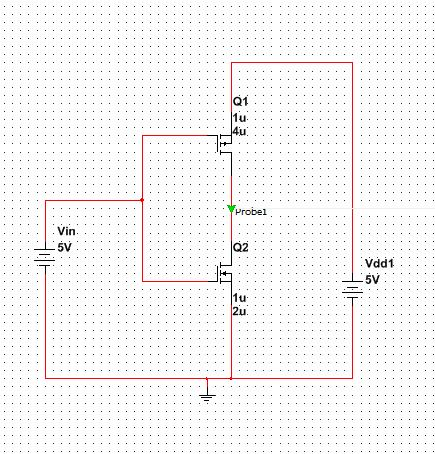
\includegraphics[width=0.5\textwidth]{5.jpg}
\caption{Schematic for CMOS inverter}
\end{figure}
\begin{itemize}
\item Create a new schematic and set up everything as shown in the diagram provided using the correct components.
\item Ensure the MOS transistors are facing the correct way, where in the case that they aren't, the can be flipped accordingly through right clicking on the component and selecting an option from the menu.
\item Set up a DC sweep for $V_{in}$ from 0-5V using an output probe of voltage as $V_O$.
\item Simulate the graph and use the cursors to obtain $V_{IL MAX}$, $V_{IH MIN}$, $V_{OL MAX}$, and $V_{OH MIN}$ at the points where the slope is tending to -1 in the appropriate regions of curvature.
\end{itemize}

\subsubsection{Results}

\begin{table}[H]
\centering
\begin{tabular}{ll}
$V_{il max}$ & 2.4V \\
$V_{ih min}$ & 2.6V \\
$V_{ol max}$ & 0.8V \\
$V_{oh min}$ & 4.2V
\end{tabular}
\caption{Static Characteristics}
\end{table}

\begin{figure}[H]
\centering
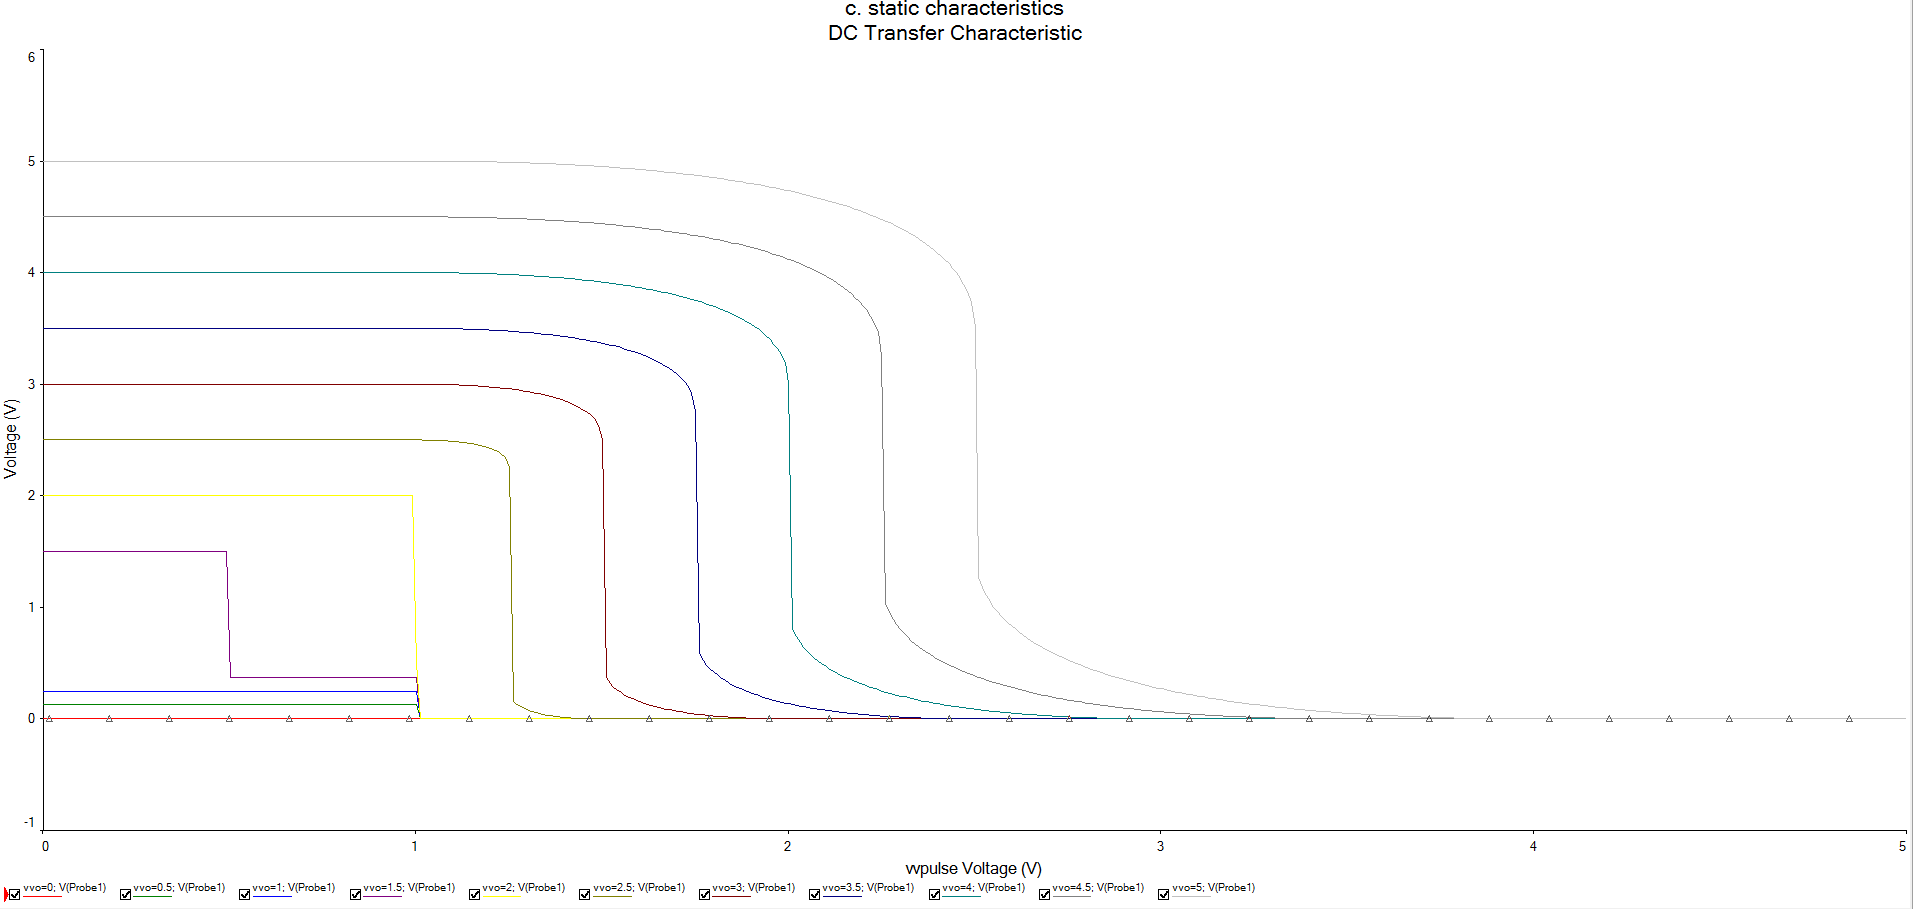
\includegraphics[width=1\textwidth]{c13.PNG}
\caption{Output of sweep, note the capacitance effect in its curvature}
\end{figure}

\subsubsection{Discussion}
CMOS is noted for its large noise margins which is demonstrated in the simulated voltage transfer characteristic with respect to voltage gain above. The voltage scaling of the inverter provides a transition from a logical high to a logical low. It is noted that at approximately 1V in the above case, the voltage reaches a threshold and begins to rapidly deteriorate in the gate characteristic. $V_{OL}$ and $V_{OH}$ are no longer at the supply rails and the transition region gain approaches 1. The result of the operation of a rapidly decreasing supply voltage that inverts the logical input. There is a growing capacitance as the voltage levels increase. This is due to the capacitative characteristics of MOS where charge can build and takes time to deplete once fully charged over a certain threshold.

\subsection{Dynamic Characteristics}
\subsubsection{Procedure}
\begin{figure}[H]
\centering
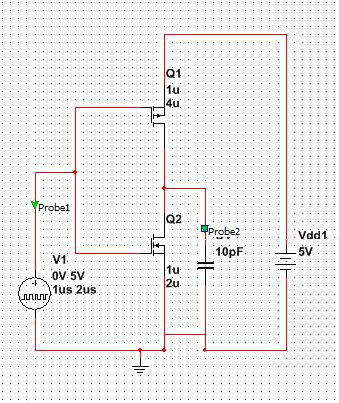
\includegraphics[width=0.5\textwidth]{6.jpg}
\caption{CMOS Dynamic Characteristics Schematic}
\end{figure}
\begin{itemize}
\item Using the schematic created in the previous part, modify the circuitry to include a capacitive dynamic condition in its configuration.
\item Using pulse voltage instead of a gate source this time, ensure the values from the image below are used.
\item Set up a transient analysis accordingly with a start time of 0, and end time of 2E-006, and a maximum time step of 4E-006.
\item Obtain the values for $t_{phl}$, $t_{plh}$, $t_f$, and $t_r$ as follows:
\begin{itemize}
\item $t_{phl}$: Input-output propagation delay at 50\% for a HI-LO transition
\item $t_{plh}$: Input-output propagation delay at 50\% for a LO-HI transition
\item $t_f$: Fall time over the 90\%-10\% HI-LO transition
\item $t_r$: Rise time over the 10\%-90\% LO-HI transition
\end{itemize}
\end{itemize}

\begin{figure}[H]
\centering
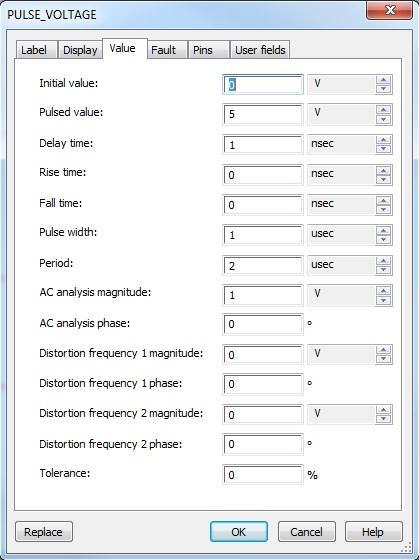
\includegraphics[width=0.5\textwidth]{8.jpg}
\caption{Output of the transient analysis}
\end{figure}

\begin{table}[H]
\centering
\begin{tabular}{ll}
$t_{PHL}$ & 0.07$\mu$s\\
$t_{PLH}$ & 81.1ns \\
$t_{f}$ & 187.1ns \\
$t_{r}$ & 1.1$\mu$s
\end{tabular}
\caption{Dynamic Characteristics}
\end{table}

\begin{figure}[H]
\centering
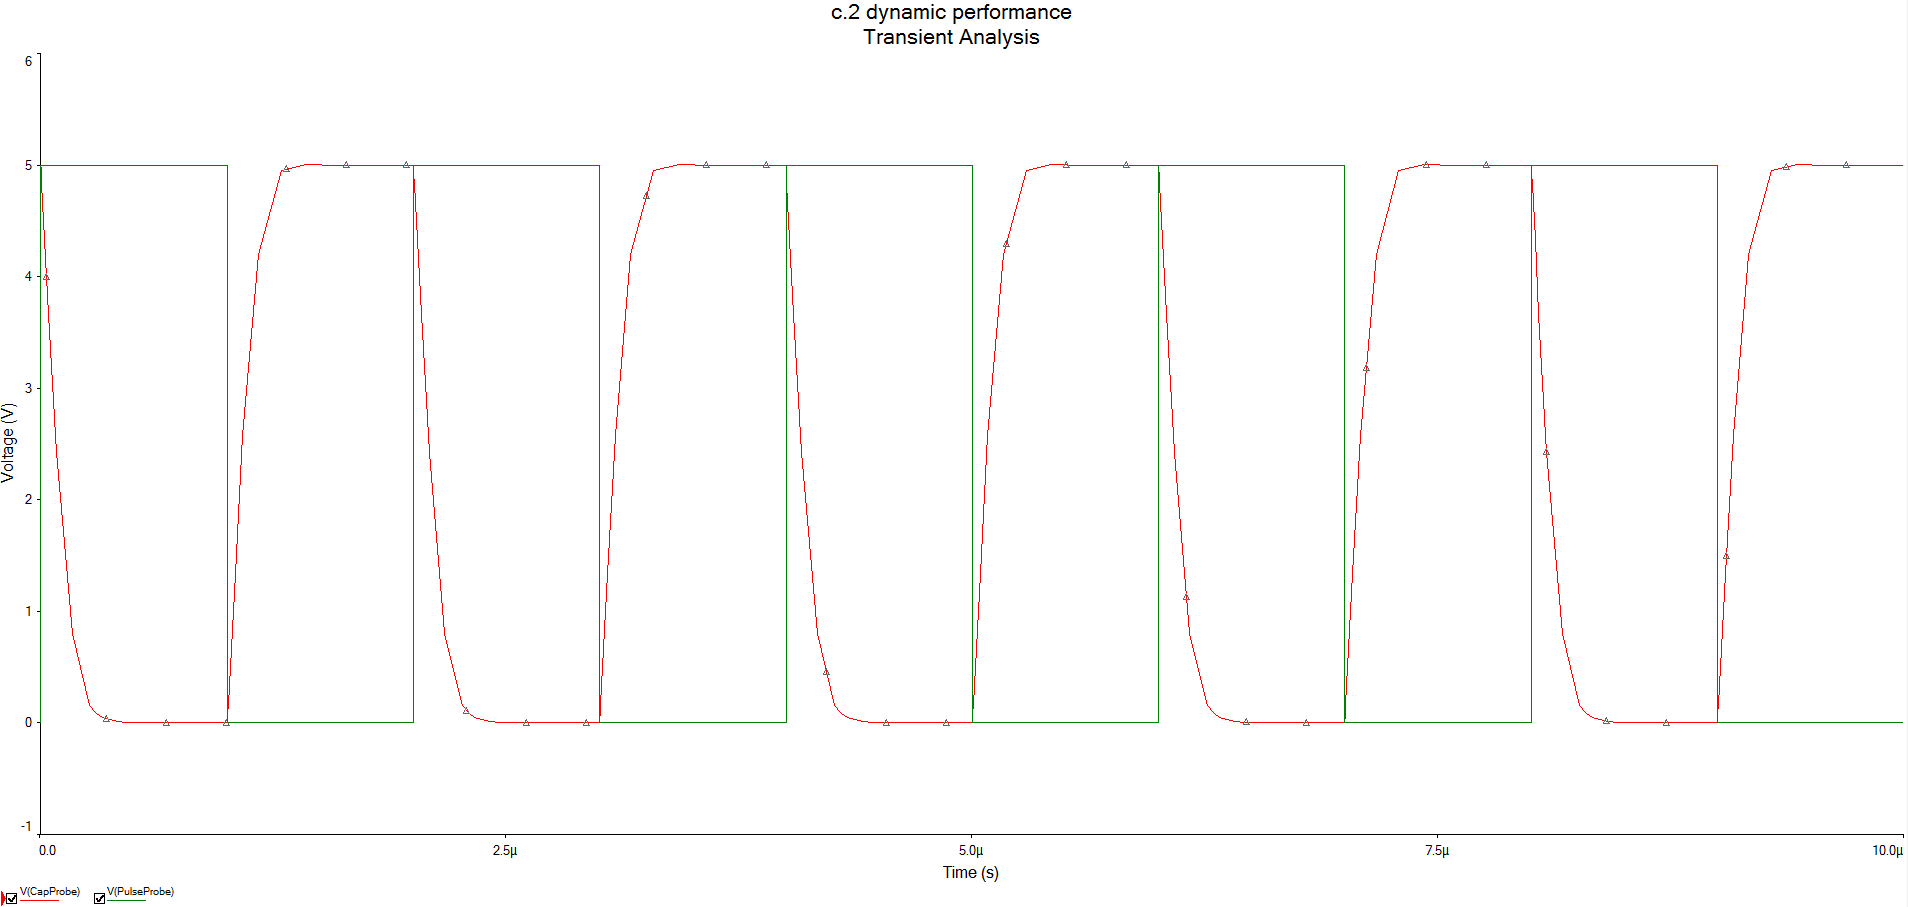
\includegraphics[width=1\textwidth]{c25.PNG}
\caption{Pulse voltage generation conditions}
\end{figure}

\subsubsection{Discussion}
The delay of the CMOS inverter is a metric of the performance of the circuit. This metric is dependent on the RC charging or discharging of the capacitative load of the MOS device. The green line in figure 10 shows the logic level provided by the source, in this case a recursive pulse voltage ranging between 0-5V ranging between a 0 and 1. The red line shows the response of the MOS transistor where the discharging time is shown by the red curve on the generation conditions. The curve is as a result of the charge held within the MOS transistor after it has reached a sufficient charge whereby a discharge must occur over an interval of time. The same is true with its charging stage, where a strong curve is formed until saturation is reached, and no further voltage is supplied over its maximum 5V. The result of this is a straight line until discharge on logical level migration.

\subsection{Discussion}
\begin{itemize}
\item What are the limitations on the accuracy of your results?
\begin{itemize}
\item Human error and eye-balling results as an approximation were major contributions to error in results as the error wasn’t entirely standard overall and the results of approximation varied per person’s
judgement.
\end{itemize}
\item How do the values of parameters compare with those obtained in the lectures?
\begin{itemize}
\item The values obtained were somewhat similar to values in lectures. There are discrepancies in values though as those in lectures are always in an ideal and theoretical environment.
\end{itemize}
\item What are the advantages or disadvantages of circuit simulations such as the one carried out in the experiment?
\begin{itemize}
\item A great advantage of such a programme would be the ability to streamline and improve the design of the circuit without too much hassle and time involved in comparison to creating and testing it out
in real life. Although these are great advantages of Multisim, a disadvantage would be that this is always in an ideal world. As we live in a world that is not always ideal, there might be some environmental factors such as temperature that would tamper with actual values.
\end{itemize}
\item What are the benefits or drawbacks of circuit simulation and of MultiSim in general as applied to the design of electronic circuits?
\begin{itemize}
\item The simulator needs to be user friendly with the graphics. It needs to be able to work efficiently and calculate the values needed at the time needed. A large library of components needs to be available to use in the simulation. All modules are accurate and up to date with the current technology. 
\end{itemize}
\item What are the essential elements of good circuit simulation and simulators?
\begin{itemize}
\item The simulator needs to be user friendly with the graphics. It needs to be able to work efficiently and calculate the values needed at the time needed. A large library of components needs to be available to use in the simulation. All modules are accurate and up to date with the current technology
\end{itemize}
\item What is the roll of the Electronic Engineer in this regard?\begin{itemize}
\item The role in this regard would be to understand how to use the software package in an efficient and educated manner. In order to do this however, a strong understanding of circuitry is required and the limits of the circuit itself.
\end{itemize}
\end {itemize}
\section{Bibliography}
\begin{thebibliography}{3}
\bibitem{streetmanb}
  Ben G. Streetman \& Sanjay Kumar Banerjee,
  \emph{Solid State Electronic Devices, 6th edition},
  Prentice Hall (2006)
\bibitem{warnerr}
  R. M. Warner Jr. \& B. L. Grung,
  \emph{MOSFET: Theory and Design},
  Oxford University Press USA (1999)
\bibitem{manom}
  M. Mano \& M. Ciletti,
  \emph{Digital Design},
  Pearson Education (2012)
\bibitem{kangs}
  S. Kang \& Y. Leblebici,
  \emph{CMOS Digital Integrated Circuits},
  McGraw Hill (1996)
\end{thebibliography}
\end{document}
